\documentclass[]{article}

\usepackage{graphicx}

\usepackage{natbib}

\usepackage{amsthm}
\usepackage{amsbsy}
\usepackage{amssymb}
\usepackage{amsfonts}
\usepackage{amssymb}
\usepackage{amsmath}
\usepackage{url}
\usepackage{paralist}
\usepackage{authblk}
\usepackage{listings}

\lstset{
	escapeinside={(*@}{@*)}
}


\bibliographystyle{chicago}

\newcommand{\currentVersion}{0.7.0}
\newcommand{\currentYear}{2018}

\title{A Guide to \textbf{Line of Sight Analyst} toolbox for ArcGIS 10.x (ver. \currentVersion{})}

\author[*]{Jan Caha}
\affil[*]{email: \textit{jan.caha@outlook.com}}


\begin{document}
\maketitle

\setcounter{tocdepth}{2}
\tableofcontents

\section{Introduction}

\textbf{Line of Sight Analyst} toolbox is a Python toolbox for ArcGIS of version 10.x. The tool aims to extend possibilities provided by existing tools \textit{Construct Sight Lines} and \textit{Line of Sight} in ArcGIS \textit{3D Analyst's Visibility toolbox}.

While \textit{Line of Sight} can be used to determine if target points are visible from observer points, which parts of the line-of-sight (LoS) are visible and invisible and where is the main obstacle located on LoS. These informations form an important part of the visibility information, however, these are often inadequate for proper assessment of visibility. Complete visibility assessment requires calculation of several LoS characteristics that can not be done by existing tools in ArcGIS.

\textbf{Line of Sight Analyst} provides tools for easier creation of LoS, analysing LoS and extracting important points from LoS. Besides these functions that are directly related to the visibility analysis the toolbox contains a tool for optimization of point location based on raster values.

\section{News}

\subsection*{ver. 0.7.0}
\begin{itemize}
	\item parameter \emph{Use earth curvature and refraction corrections?} is now by default checked for all tools
\end{itemize}

\subsection*{ver. 0.6.7}
\begin{itemize}
	\item bug fixed in elevation difference to global horizon calculation
\end{itemize}

\subsection*{ver. 0.6.6}
\begin{itemize}
	\item minor bug fixes and description texts clarification.
\end{itemize}

\subsection*{ver. 0.6.0}
\begin{itemize}
	\item added Earth curvature and atmospheric refraction corrections for all relevant tools
\end{itemize}

\subsection*{ver. 0.5.1}
\begin{itemize}
	\item first public release
\end{itemize}

\section{Tools}

The toolbox contains 8 tools:
\begin{itemize}
	\item Optimize Point Location,
	\item Create Lines of Sight,
	\item Create Global Lines of Sight,
	\item Analyse Lines of Sight,
	\item Analyse Global Lines of Sight,
	\item Extract Local Horizons,
	\item Extract Global Horizon,
	\item Export Line of Sight into CSV.
\end{itemize}
The typical workflow of the toolbox is show in Fig. \ref{Fig:Workflow}.

\begin{figure}
	\centering
	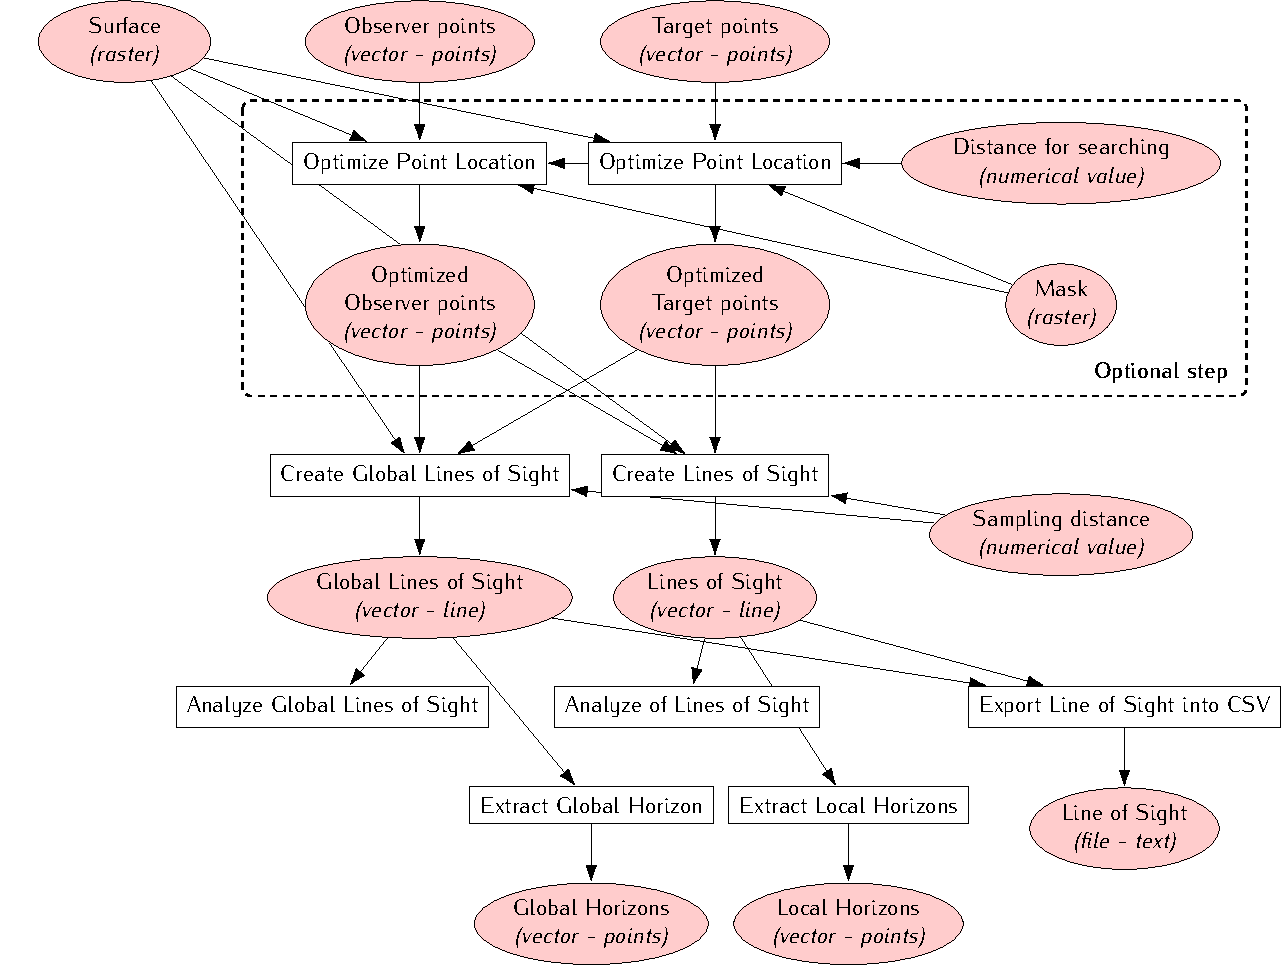
\includegraphics[width=\textwidth]{./images/workflow.pdf}
	\caption {Typical workflow when using \textbf{Line of Sight Analyst}.}
	\label{Fig:Workflow}
\end{figure} 

\subsection{Optimize Point Location}

A tool designed for optimization of point location with respect to values of the raster. The tool selects highest value of the raster within the distance for searching and moves the point to that location. The higher value of the raster is likely to point at locations with higher visibility potential. However, in some cases the higher raster values do not necessarily lead to better visibility. This is caused by the fact that the visibility is affected by many parameters and thus it is quite problematic to properly optimize point's locations.

The optimization can be based on elevation or other surface characteristics like positive openness or local dominance that are implemented in \textit{Relief Visualization Toolbox} \citep{Kokalj2016}.

\subsubsection{Parameters}
\begin{itemize}
	\item \textbf{Optimization raster} - \textit{raster} - layer that is used to optimize point location (e.g. elevation, local dominance, positive openness or some other characteristics)
	\item \textbf{Points to be optimized} - \textit{features - points} - points which location should be optimized
	\item \textbf{Distance for searching} - \textit{numerical value} - distance around points in which the better positions are searched. (The higher the value the longer the running time of the tool!)
	\item \textbf{Optimized points} - \textit{features - points} - output layer of optimized points.
	\item \textbf{Use mask?} - \textit{boolean} - variable that defines if the mask for point's location should be used.
	\item \textbf{Mask} - \textit{raster} - raster where values higher then zero specifies locations that can be used for point location. Values lower or equal to zero define areas that can not be used for points.
\end{itemize}

\subsubsection{Output}

New point feature class with points moved to optimized locations.

\subsection{Create Lines of Sight}
\label{Sec:createLoS}
A tool used to create Lines of Sight amongst observer and target points. Offsets of both observer and target points are specified as fields to allow individual setting for each point. LoS are created between every observer and target point which means that if there are $n$ observer points and $m$ target ponts then there will be $n \times m$ lines-of-sight.

\subsubsection{Parameters}
\begin{itemize}
	\item \textbf{Surface} - \textit{raster} - surface on which the LoS are determined.
	\item \textbf{Observer points} - \textit{features - points} - locations of observing points.
	\item \textbf{Observer points offset} - \textit{field - double} - field of the layer Observer points that has data type Double. The parameter specifies vertical offset of the observer from the surface.
	\item \textbf{Target points} -  \textit{features - points} - locations of target points.
	\item \textbf{Target points offset} - \textit{field - double} - field of the layer Target points that has data type Double. The parameter specifies vertical offset of the observer from the surface. 
	\item \textbf{Sampling distance} - \textit{numeric value} - value in units specified by Surface coordinate system that determines how often the points are placed on LoS. Default value is the same as cellsize of Surface.
	\item \textbf{Output feature layer} - \textit{features - lines} - output layer.
\end{itemize}

\subsubsection{Output}

Line feature class with lines-of-sight, that has Z-dimension. Specific fields are \textit{OID\_OBSERV}, \textit{observ\_offset}, \textit{OID\_TARGET} and \textit{target\_offset} which are necessary for further analyses. The geometry store coordinates (X,Y and Z) purely from the surface without the offsets which are stored in fields.

\subsection{Create Global Lines of Sight}

This tool is basically the same as \textbf{Create Lines of Sight} (sec. \ref{Sec:createLoS}) but creates LoS that does not end at target point but goes beyond it and ends at extent of the surface used to define LoS.

\subsubsection{Parameters}
The same as for \textbf{Create Lines of Sight} (sec. \ref{Sec:createLoS}).

\subsubsection{Output}

The same as for \textbf{Create Lines of Sight} (sec. \ref{Sec:createLoS}).

Since the global LoS does not end at the target point two more fields are necessary to store position of target point on the LoS. Fields \textit{target\_x} and \textit{target\_y} store coordinates of the target point for LoS and are necessary for further calculations.


\subsection{Export Line of Sight into CSV}

A tool for exporting LoS into format that can be processed outside ArcGIS.

\subsubsection{Parameters}
\begin{itemize}
	\item \textbf{Lines of Sight} - \textit{features - lines} - layer containing LoS.
	\item \textbf{Line of Sight ID} - \textit{id} - ID of the LoS to be exported.
	\item \textbf{Output file} - \textit{file} - name and locations of the CSV that will be created.
	\item \textbf{Include offsets?} -  \textit{boolean} - export only LoS without observer and target offsets or include the offsets in LoS? Default value is to include the offsets.
	\item \textbf{Global Line of Sight?} - \textit{boolean} - is the LoS global? The tool tries to determine if the LoS is global based on typical fields. Warning message is shown if the tool determines that the LoS is global and this option is not checked. Default value is false.
	\item \textbf{Observer point offset} - \textit{field - double} - field of the layer Lines of Sight that has data type Double. If the field has default name (\textit{observ\_offset}) from tools in this toolbox then it is selected automatically.
	\item \textbf{Target point offset} - \textit{field - double} - field of the layer Lines of Sight that has data type Double. If the field has default name (\textit{target\_offset}) from tools in this toolbox then it is selected automatically.
	\item \textbf{Target point X coordinate} - \textit{field - double} - field of the layer Lines of Sight that has data type Double. If the field has default name (\textit{target\_x}) from tools in this toolbox then it is selected automatically.
	\item \textbf{Target point Y coordinate} - \textit{field - double} - field of the layer Lines of Sight that has data type Double. If the field has default name (\textit{target\_y}) from tools in this toolbox then it is selected automatically.
	\item \textbf{Use earth curvature corrections?} - \textit{boolean} - should Earth's curvature and refraction corrections be used? Default value is yes.
	\item \textbf{Refractivity coefficient} - \textit{numerical value}  - coefficient value (default 0.13).
\end{itemize}

Parameters \textbf{Observer point offset} and \textbf{Target point offset} are summarized in parameter group \textbf{Offsets}, parameters \textbf{Target point X coordinate} and \textbf{Target point Y coordinate} in parameter group \textbf{Global Line of Sight} and parameters \textbf{Use earth curvature corrections?} and \textbf{Refractivity coefficient} in parameter group \textbf{Curvature corrections}.

\subsubsection{Output}

CSV file delimited by ";" with header "distance";"elevation" if LoS is local and "distance";"elevation";"target point"  if the LoS is global. Field "target point" have value 1 if the point is target point and 0 otherwise.

\subsection{Analyze of Lines of Sight}

A tool used to analyse LoS. The tool should be used only on local LoS that connect observer points with target points. There is another tool for analyses of Global LoS.

\subsubsection{Parameters}
\begin{itemize}
	\item \textbf{Lines of Sight} - \textit{features - lines} - layer containing LoS.
	\item \textbf{Observer points offset} - \textit{field - double} - field of the layer Lines of Sight that has data type Double. If the field has default name (\textit{observ\_offset}) from tools in this toolbox then it is selected automatically.
	\item \textbf{Target points offset} - \textit{field - double} - field of the layer Lines of Sight that has data type Double. If the field has default name (\textit{target\_offset}) from tools in this toolbox then it is selected automatically.
	\item \textbf{Object size} - \textit{numeric value} - size of the theoretical observed object.
	\item \textbf{Recognition acuinty} - \textit{numerical value} - recognition acuinty of the observer's eye. Default value is $1^\prime$ or $1/60$ of degree which equals to 0.017. 
	\item \textbf{Clear visibility distance limit} - \textit{numerical value} - maximal distance on which the user can absolutely clearly see the object with Object size.
	\item \textbf{Use earth curvature corrections?} - \textit{boolean} - should Earth's curvature and refraction corrections be used? Default value is yes.
	\item \textbf{Refractivity coefficient} - \textit{numerical value}  - coefficient value (default 0.13).
\end{itemize}

Parameters \textbf{Object size}, \textbf{Recognition acuinty} and \textbf{Clear visibility distance limit} are summarized in parameter group \textbf{Fuzzy visibility} as they are related to fuzzy visibility calculation only. Parameters \textbf{Use earth curvature corrections?} and \textbf{Refractivity coefficient} in parameter group \textbf{Curvature corrections}.

\subsubsection{Output}

A set of new fieds for the layer \textbf{Lines of Sight}:
\begin{itemize}
	\item \textbf{Visible} - \textit{Short} - value indicating if the target point is visible (1) or invisible (0).
	\item \textbf{ViewAngle} - \textit{Double} - vertical viewing angle from observer to target. Units are degrees.
	\item \textbf{ElevDiff} - \textit{Double} - vertical difference amongst observer and target, negative value indicates that observer is lower then target. Units are the same as used in \textbf{Lines of Sight}.
	\item \textbf{AngleDiff\_H} - \textit{Double} - angle difference between viewing angle of target and highest horizon on the LoS. Negative value indicates that the horizon hides target point, possitive value indicates how high above the horizon the target rises. Units are degrees.
	\item \textbf{ElevDiff\_H} - \textit{Double} - elevation difference between target point and highest horizon on the LoS. Possitive value indicates how much of the target is visible (from the top towards bottom), negative value indicates how much higher the target had to be to be visible for the observer. Units are the same as used in \textbf{Lines of Sight}.
	\item \textbf{SlopeDiff} - \textit{Double} - difference between viewing angle from observer to target and slope of LoS towards target. The closer the value to $90^\circ$ the better for observer as the target is more significant. Units are degrees.
	\item \textbf{Horizon\_C} - \textit{Short} - number of visible horizons located between observer and target.
	\item \textbf{HorDist} - \textit{Double} - distance from observer to the highest horizon on the LoS. Units are the same as used in \textbf{Lines of Sight}.
	\item \textbf{FuzzyVis} - \textit{Double} - fuzzy visibility value indicating distinctiveness of the object defined by Fuzzy visibility parameters. Distinctiveness is best if the value is 1 and gets worser as the value approaches 0. For detailed description of fuzzy visibility please take a look at publications by \cite{Fisher1994} and \cite{Ogburn2006}.
\end{itemize}

\subsection{Analyze Global Lines of Sight}

A tool used to analyse Global LoS. The tool should not be used for local LoS that connect only observer to target.

For purpose of these analyses the target point can not be a global horizon. This assumption allows to properly calculate all the characteristics of global LoS.

\subsubsection{Parameters}
\begin{itemize}
	\item \textbf{Global Lines of Sight} - \textit{features - lines} - layer containing LoS.
	\item \textbf{Observer points offset} - \textit{field - double} - field of the layer Lines of Sight that has data type Double. If the field has default name (\textit{observ\_offset}) from tools in this toolbox then it is selected automatically.
	\item \textbf{Target points offset} - \textit{field - double} - field of the layer Lines of Sight that has data type Double. If the field has default name (\textit{target\_offset}) from tools in this toolbox then it is selected automatically.
	\item \textbf{Target point X coordinate} - \textit{field - double} - field of the layer Lines of Sight that has data type Double. If the field has default name (\textit{target\_x}) from tools in this toolbox then it is selected automatically.
	\item \textbf{Target point Y coordinate} - \textit{field - double} - field of the layer Lines of Sight that has data type Double. If the field has default name (\textit{target\_y}) from tools in this toolbox then it is selected automatically.
	\item \textbf{Use earth curvature corrections?} - \textit{boolean} - should Earth's curvature and refraction corrections be used? Default value is yes.
	\item \textbf{Refractivity coefficient} - \textit{numerical value}  - coefficient value (default 0.13).
\end{itemize}

Parameters \textbf{Use earth curvature corrections?} and \textbf{Refractivity coefficient} in parameter group \textbf{Curvature corrections}.

\subsubsection{Output}

A set of new fieds for the layer \textbf{Global Lines of Sight}:
\begin{itemize}
	\item \textbf{Visible} - \textit{Short} - value indicating if the target point is visible (1) or invisible (0).
	\item \textbf{ViewAngle} - \textit{Double} - vertical viewing angle from observer to target. Units are degrees.
	\item \textbf{ElevDiff} - \textit{Double} - vertical difference amongst observer and target, negative value indicates that observer is lower then target. Units are the same as used in \textbf{Lines of Sight}.
	\item \textbf{AngleDiff\_GH} - \textit{Double} - angle difference between viewing angle of target and the global horizon on the LoS. Negative value indicates that the horizon is higher then target point, possitive value indicates that target point is highest point on LoS. Negative value does not mean that the target point is invisible as the global horizon can be located behind the target point. Units are degrees.
	\item \textbf{ElevDiff\_GH} - \textit{Double} - elevation difference between target point and global horizon on the LoS. Positive value indicates how much of the target is visible against sky (from the top towards bottom), negative value indicates how much higher the target had to be to reach global horizon. Units are the same as used in \textbf{Lines of Sight}.
	\item \textbf{HorDist} - \textit{Double} - distance between global horizon and target point. Negative value means that global horizon is located before target point, positive value means that it is located behind the target. 
	\item \textbf{Horizon\_C} - \textit{Short} - number of visible horizons located behind target point.
\end{itemize}


\subsection{Extract Local Horizons}

A tool used to extract visible horizons from local LoS. 

\subsubsection{Parameters}
\begin{itemize}
	\item \textbf{Lines of Sight} - \textit{features - lines} - layer containing LoS.
	\item \textbf{ID observer} - \textit{Short} - field of the layer \textbf{Lines of Sight} that has data type Short. If the field has default name (\textit{OID\_OBSERV}) from tools in this toolbox then it is selected automatically.
	\item \textbf{Observer points offset} - \textit{field - double} - field of the layer \textbf{Lines of Sight} that has data type Double. If the field has default name (\textit{observ\_offset}) from tools in this toolbox then it is selected automatically.
	\item \textbf{ID target} - \textit{Short} - field of the layer \textbf{Lines of Sight} that has data type Short. If the field has default name (\textit{OID\_TARGET}) from tools in this toolbox then it is selected automatically.
	\item \textbf{Target points offset} - \textit{field - double} - field of the layer \textbf{Lines of Sight} that has data type Double. If the field has default name (\textit{target\_offset}) from tools in this toolbox then it is selected automatically.
	\item \textbf{Output feature layer} - \textit{features - points} - output layer.
	\item \textbf{Use earth curvature corrections?} - \textit{boolean} - should Earth's curvature and refraction corrections be used? Default value is yes.
	\item \textbf{Refractivity coefficient} - \textit{numerical value}  - coefficient value (default 0.13).
\end{itemize}

\subsubsection{Output}

Point feature class containing horizons, that has Z-dimension. The feature class has fields that allow connection with observer points (\textit{OID\_OBSERV}), target points (\textit{OID\_TARGET}) and also LoS (\textit{OID\_LoS}). 

Besides that there are several attributes of horizons:
\begin{itemize}
	\item \textbf{Hor\_Type} - \textit{Short} - value indicating if the horizon is highest horizon of LoS (value 1) or not (value 0).
	\item \textbf{Hide\_Tar} - \textit{Short} - value indicating if the horizon hides target (1) or if the target would be visible behind this horizon (0).
	\item \textbf{ViewAngle} - \textit{Double} - viewing angle between observer point and the horizon.
	\item \textbf{AngleDiff\_H} - \textit{Double} - angle difference between viewing angle of this horizon and previous horizon. Value zero means that there is no previous horizon.
	\item \textbf{Dist\_Observ} - \textit{Double} - distance from horizon to the observer.
\end{itemize}

\subsection{Extract Global Horizon}

A tool used to extract visible global horizon from global LoS. 

\subsubsection{Parameters}
\begin{itemize}
	\item \textbf{Global Lines of Sight} - \textit{features - lines} - layer containing global LoS.
	\item \textbf{ID observer} - \textit{Short} - field of the layer \textbf{Lines of Sight} that has data type Short. If the field has default name (\textit{OID\_OBSERV}) from tools in this toolbox then it is selected automatically.
	\item \textbf{Observer points offset} - \textit{field - double} - field of the layer \textbf{Lines of Sight} that has data type Double. If the field has default name (\textit{observ\_offset}) from tools in this toolbox then it is selected automatically.
	\item \textbf{ID target} - \textit{Short} - field of the layer \textbf{Lines of Sight} that has data type Short. If the field has default name (\textit{OID\_TARGET}) from tools in this toolbox then it is selected automatically.
	\item \textbf{Target points offset} - \textit{field - double} - field of the layer \textbf{Lines of Sight} that has data type Double. If the field has default name (\textit{target\_offset}) from tools in this toolbox then it is selected automatically.
	\item \textbf{Target point X coordinate} - \textit{field - double} - field of the layer Lines of Sight that has data type Double. If the field has default name (\textit{target\_x}) from tools in this toolbox then it is selected automatically.
	\item \textbf{Target point Y coordinate} - \textit{field - double} - field of the layer Lines of Sight that has data type Double. If the field has default name (\textit{target\_y}) from tools in this toolbox then it is selected automatically.
	\item \textbf{Output feature layer} - \textit{features - points} - output layer.
	\item \textbf{Use earth curvature corrections?} - \textit{boolean} - should Earth's curvature and refraction corrections be used? Default value is yes.
	\item \textbf{Refractivity coefficient} - \textit{numerical value}  - coefficient value (default 0.13).
\end{itemize}

\subsubsection{Output}

Point feature class containing global horizons, that has Z-dimension. The feature class has fields that allow connection with observer points (\textit{OID\_OBSERV}), target points (\textit{OID\_TARGET}) and also LoS (\textit{OID\_LoS}). 

Besides that there are several attributes of horizons:
\begin{itemize}
	\item \textbf{Hide\_Tar} - \textit{Short} - value indicating if the horizon hides target (1) or if the target would be visible behind this horizon (0).
	\item \textbf{ViewAngle} - \textit{Double} - viewing angle between observer point and the horizon.
	\item \textbf{AngleDiff\_Tar} - \textit{Double} - angle difference between viewing angle of this horizon and target point. 
	\item \textbf{Dist\_Observ} - \textit{Double} - distance from horizon to the observer.
	\item \textbf{Behind\_Tar} - \textit{Short} - value indicating if the horizon is behind target (1) or before target point (0).
\end{itemize}

\section{Known Issues}

\begin{itemize}
	\item No issues are known at this time.
\end{itemize}

\section{Solved Issues}

\begin{itemize}
	\item prior to version 0.6.6 \textbf{ElevDiff\_GH} (elevation difference between target point and global horizon on the LoS) was not calculated correctly
\end{itemize}

\section{Future Plans}

\begin{itemize}
	\item Future versions will include suggestions from users and testers, if there will be any.
	\item There plans for tools that would deal with linear horizons (definition, extraction from the surface and evaluation).
\end{itemize}

\section{Citation}

If you use this toolbox in publication, please consider using this citation of my work. 
\vspace{1em}

\noindent Cite as:
\vspace{1em}

\noindent Caha, Jan. \currentYear{}. “A Guide to Line of Sight Analyst Toolbox for ArcGIS 10.x (ver. \currentVersion{}).”  \url{https://jancaha.github.io/Line-of-Sight-Analyst/assets/files/Line\_of\_Sight\_Analyst.pdf}.
\vspace{1em}

\noindent or in bibtex:
\vspace{1em}
\begin{lstlisting}
@TechReport{LoSAnalyst,
author = {Jan Caha},
title  = {Line of Sight Analyst toolbox for ArcGIS 10.x
         (ver. (*@\currentVersion{}@*))},
year   = {(*@\currentYear{}@*)},
url    = {https://jancaha.github.io/Line-of-Sight-Analyst/
          assets/files/Line_of_Sight_Analyst.pdf},
}
\end{lstlisting}

\vspace{1em}

\noindent Thank you!

\bibliography{bibliography}

\end{document}        